\chapter{Line Following Robot} \label{chap:lineFollowingRobot}
\section{Case Description} The line following robot is a
co-model that demonstrates how design space exploration is supported
in \DESTECS.  The co-model simulates a robot that can follow a line
painted on the ground. It is assumed that the colour of the line is
known and that it is differentiated from the background colour (which
is not known), but the line may exhibit gentle or sharp corners or
angled corners in any direction. The robot uses a number of sensors to
detect light and dark areas on the ground and has two wheels, each
powered individually with motors to enable the robot to make
fine-graded changes in direction.

\begin{figure}[htb!]
\begin{center}
\subfigure[An R2-G2P robot]
{
      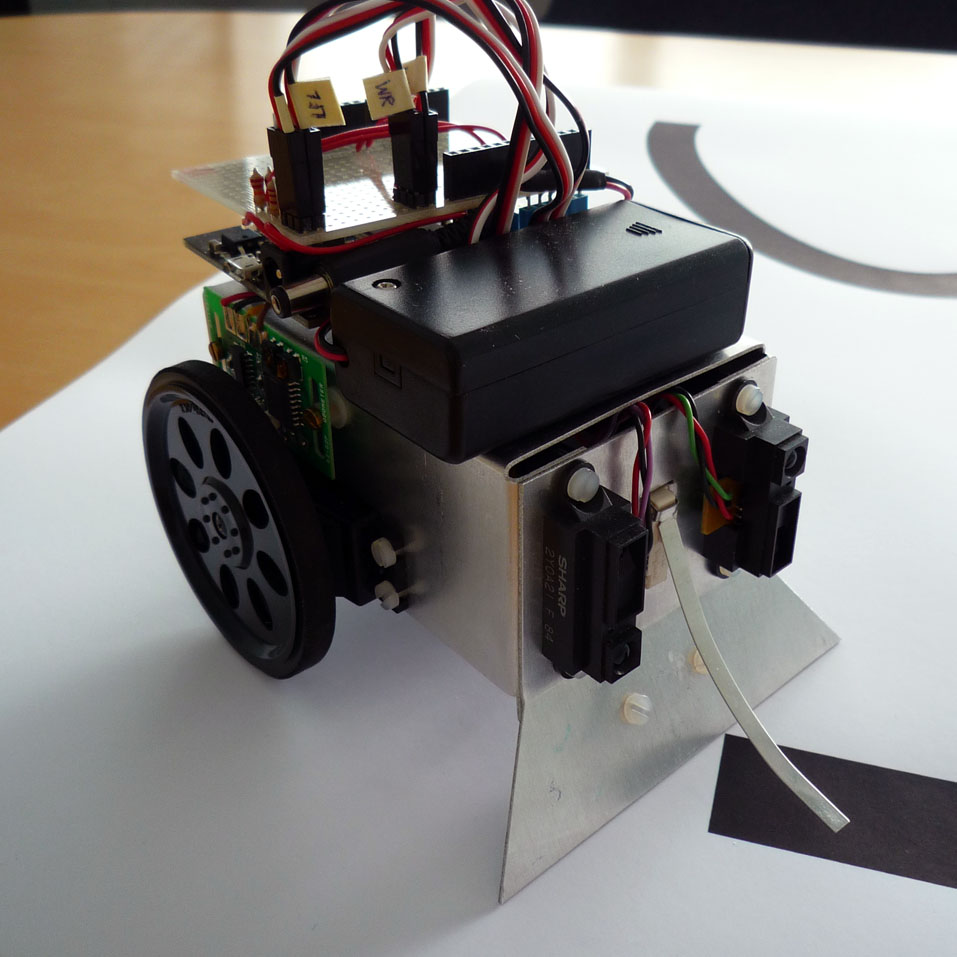
\includegraphics[width=0.3\linewidth]{lineFollowingRobot/r2g2p_netduino}
      \label{fig:r2g2p_sm}
}
\subfigure[A line-follow path]
{
      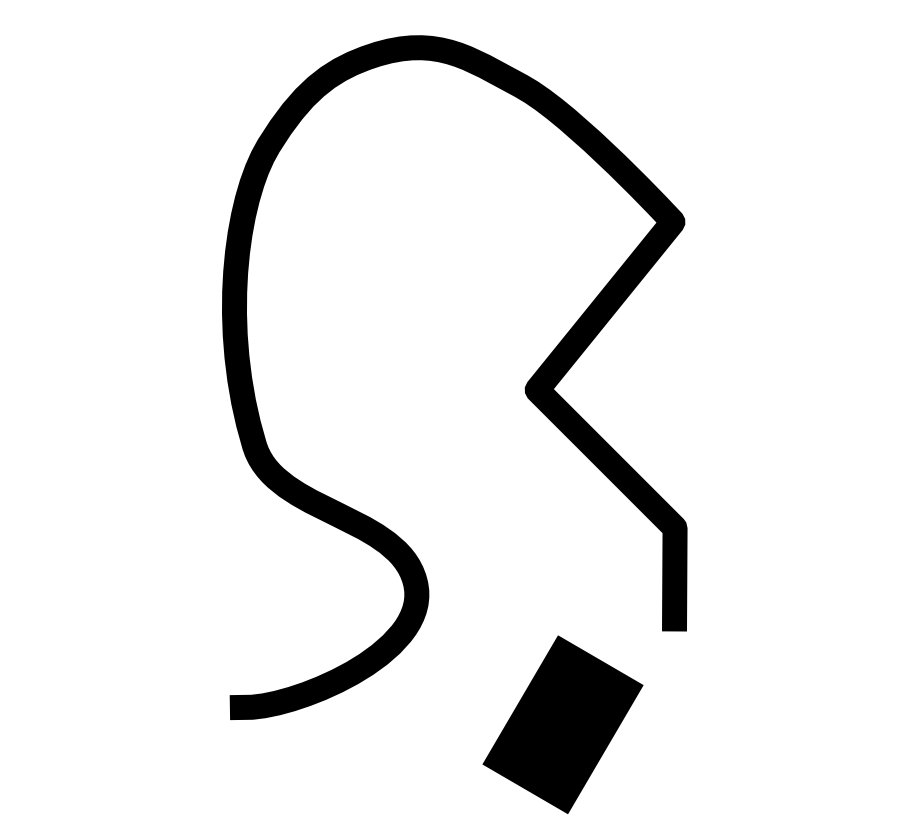
\includegraphics[width=0.3\linewidth]{lineFollowingRobot/map}
      \label{fig:r2g2p_3dpath}
}
\subfigure[3D representation of the R2-G2P]
{
      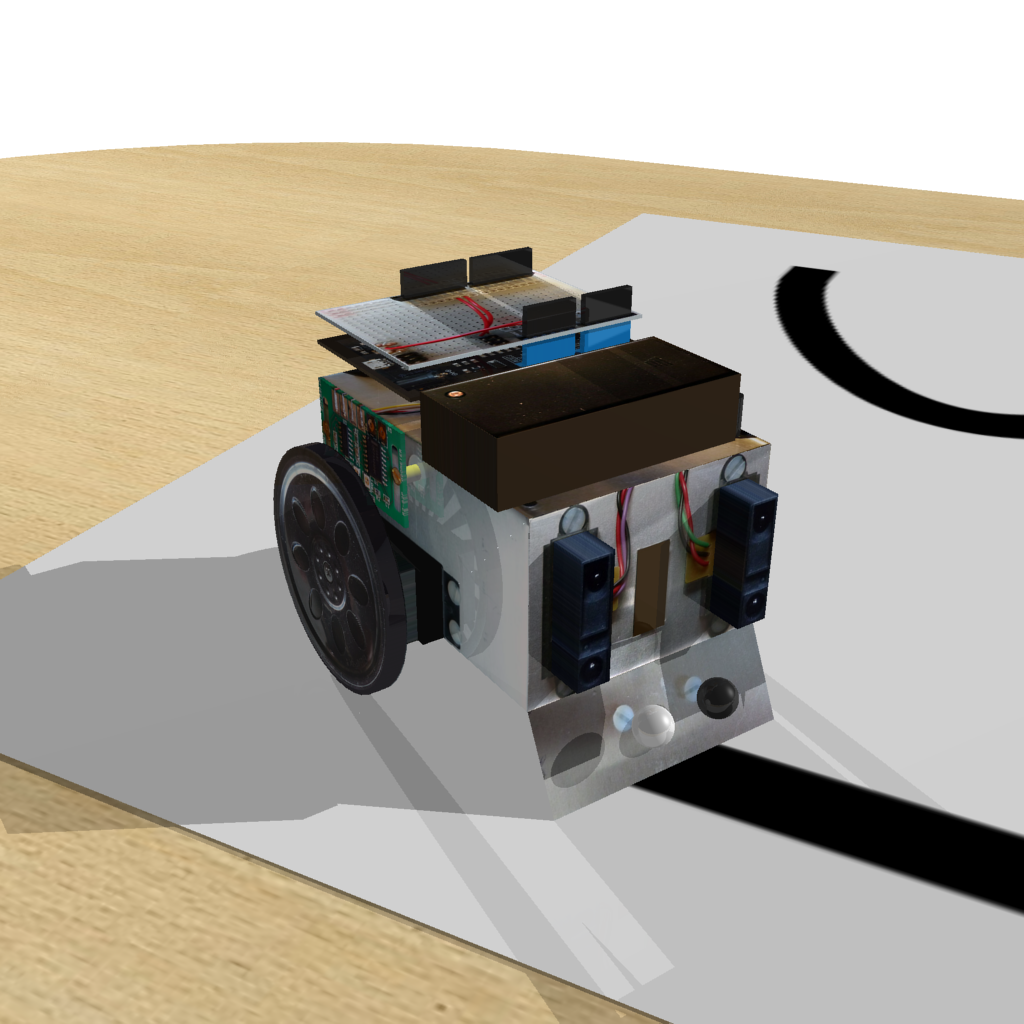
\includegraphics[width=0.3\linewidth]{lineFollowingRobot/robot_inside}
      \label{fig:r2g2p_3d}
}
\caption{The line-following robot}
\label{fig:r2g2p_study}
\end{center}
\end{figure}

There are a number of design decisions to make when designing the
robot.  For example, possible variations might include changing the
number of sensors or changing their positions (sensor position can be
adjusted laterally or longitudinally). Any given design can be
assessed by comparing distance travelled, which will be shorter for
more accurate robots, and average speed, which will ideally be as high
as possible.  \DESTECS facilitates exploration of the design space by
automating simulations with different design parameters. For example,
\DESTECS can automatically simulate a model with two sensors set
initially close together, then increasing the distance between them by
some distance \texttt{n} until a maximum distance is reached.  The
results of each simulation can then be compared to determine the ideal
robot design.

The co-model supplied here uses two sensors to detect light and dark,
and two motors (one for each wheel).  Two encoders (also one for each
wheel) close the feedback loop so that actual wheel rotations can be
monitored and the output to the motors adjusted accordingly.

The robot moves through a number of phases as it follows a line.  At
the start of each line is a specific pattern that will be known in
advance.  Once a genuine line is detected on the ground, the robot
follows it until it detects that the end of the line has been reached,
when it should go to an idle state.  For modelling purposes the
co-model accepts a textual representation of a bitmap as the surface with a line to be followed.

%\fbox{Can we insert a figure here?}
%\section{External links}


%-- shared design parameters
%sdp real wheel_radius;
%sdp real encoder_resolution;
%sdp real line_follow_x;
%sdp real line_follow_y;
%sdp array initial_position[3];
%sdp real fast_wheel_speed;
%sdp real slow_wheel_ratio;
%
%-- encoders
%monitored real encoder_left;
%monitored real encoder_right;
%
%-- line-following sensors
%monitored real lf_left;
%monitored real lf_right;
%
%-- line-following sensor fail flags
%monitored bool lf_left_fail_flag;
%monitored bool lf_right_fail_flag;
%
%-- servos
%controlled real servo_left;
%controlled real servo_right;

\section{Contract}
The contract contains eight shared variables.  Two \emph{controlled}
variables of type \keyw{real} produce signals for the actuators that
power the motors for the left (\texttt{servo\_left}) and right
(\texttt{servo\_right}) wheels.  And two \emph{monitored}
variables of type \keyw{real} are used to feed back information about
the rotations of the left (\texttt{encoder\_left}) and right
(\texttt{encoder\_right}) wheels.

Two \emph{monitored} variables of type \keyw{real} are used to represent
inputs from line-following sensors that can detect areas of light and
dark on the ground.  In this model there are two sensors,
\texttt{lf\_left} and \texttt{lf\_right}, but other models may carry more
or fewer line-following sensors.

Two \emph{monitored} variables of type \keyw{bool} are used to indicate
 whether a fault has been detected on the left wheel
 (\texttt{lf\_left\_fail\_flag}) or right wheel
 (\texttt{lf\_right\_fail\_flag}).  It is assumed that the CT model can
 self-detect and report some faults to the DE model.

%And finally, a single \emph{controlled} variable of type \keyw{matrix} is
%contained in the contract to represent an array of LEDs \texttt{leds}.
%The LEDs could be used to indicate the current state of the controller
%visually (e.g., in a 3D visualisation).

The contract also includes seven \emph{shared design parameters}: wheel radius, in metres (\texttt{wheel\_\-radius})); encoder resolution, in counts per revolution (\texttt{encoder\_resolution}); the separation of the line-following sensors from the centre line, in metres (\texttt{line\_follow\_x}); distance forward of the line-following sensors from the centre of the robot, in metres (\texttt{line\_follow\_y}); an array giving initial position \texttt{x}, \texttt{y}, \texttt{theta} (\texttt{initial\_position[3]}); and two shared variables representing controller aggression in terms of maximum wheel speed (\texttt{fast\_wheel\_speed}) and turn ratio (\texttt{slow\_wheel\_ration}), both in the range [0,1].

\section{Discrete-event}

The DE model makes heavy use of inheritance, providing abstract
classes for controller, sensors and actuators. The servos are accessed through objects of the \texttt{SpeedServo} class, which inherits from the \texttt{IActuatorRealPercent}; and the encoders are read through objects of the \texttt{Encoder} class, which inherits from the \texttt{ISensorReal}.

The line-following sensors make greater use of the benefits of inheritance. The raw sensor readings are accessed through objects of the \texttt{IRSensor} class, which inherits from the \texttt{ISensorInt8} class. Because the CT model of the line-following sensors includes sensor noise, the \texttt{Filtered\-IR\-Sensor} is used. This class contains an \texttt{IRSensor} and maintains a floating average using the last five sensor readings. This class also inherits from the \texttt{ISensorInt8}, which means that an \texttt{IRSensor} object can be swapped for a filtered object seamlessly. This is an example of the standard \emph{decorator} pattern~\cite{DESIGNPAT95}.

As mentioned above, the sensors are calibrated to set when it is considered to be reading black. This can change if the ambient light is increased in the model. The calibration is set in a \texttt{BlackWhiteSensor} class, which holds an \texttt{IRSensor} object and has Boolean operations to determine if the sensor is seeing black or white.

The controller is modal, meaning that with each `phase' (initialisation, sensor calibration, line-following, etc.) is realised as a mode, represented by the \texttt{IMode} interface. This interface defines four operations: \texttt{Enter}, called when the controller changes to this mode; \texttt{Step()}, called each control cycle; \texttt{Exit()}, called when the controller finishes this mode; and \texttt{Done()}, which allows a mode to indicate it has finished its task. The two abstract classes \texttt{AbstractMode} and \texttt{AbstractModeTimed} provide empty implementations of these operations. The timed mode keeps track of how long it has been running, and \texttt{Done()} will yield \texttt{\textbf{true}} after a specified time.

The top-level controller class is the \texttt{AbstractModalController}. This class holds a reference to each sensor object and provides getter methods to access these objects. The abstract mode classes hold a reference to the \texttt{AbstractModalController}, so that each mode can access the sensors and actuators. The \texttt{LineFollower} class is a subclass of this class, which instantiates the modes it requires to follow the line, which are held in a map. The identifier of the current mode is recorded in the \texttt{mode} variable and modes are changed with the \texttt{ChangeMode} operation. The \texttt{CheckModeChange} operation contains the logic for changing mode.

The following modes are followed in order: \texttt{WaitMode}, which gives the sensors time to start up; \texttt{CalibrateMode}, which calibrates the sensors using the predetermined starting pattern; \texttt{FindLineMode}, which drives forward until the line is found; and finally \texttt{FollowMode}, which follows the line.

If one of the sensors fails, the controller switched to  \texttt{SingleFollowMode}, which uses the one remaining working sensor to follow the line. Modes can also cause a change of mode by returning the identifier of a mode from the \texttt{Step()} operation. This functionality is used by the \texttt{SingleFollowMode} class to switch to \texttt{RefindLineMode} when it loses the line. The \texttt{RefindLineMode} sweeps back and forth until it sees black, then returns to \texttt{Single\-Follow\-Mode}.

The \texttt{System} class instantiates the
\texttt{LineFollower} object and deploys it to a single CPU. All sensor and actuator objects are created in the \texttt{IOFactory} class, which provides so-called ``factory'' methods that return the requested sensors. The \texttt{IOFactory} object is created in the \texttt{System} class and passed to the \texttt{LineFollower} object. The periodic thread is defined in the \texttt{Thread} class. This class holds a reference the controller and IO factory. This means that all the sensors and actuators can be synchronised at once, then the controller is called. This improves simulation speed.



\section{Continuous-time}

The CT model (pictured in Figure~\ref{fig:r2g2p_study}) is broken down into blocks that broadly represent physical components. The central \emph{body} block is a bond graph representation of the physics, with bond graph models of the wheels (\emph{wheel\_left, wheel\_right}) and servos (\emph{servo\_left, servo\_right}) connected on either side. The encoder blocks (\emph{encoder\_left, encoder\_right}) produce 44 counts per revolution of the wheel. Two line-following sensor blocks (\emph{lf\_left}, \emph{lf\_right}) are also connected to the body, as well a \emph{map} block. The encoder, line-following sensor and servo blocks are all connected to a \emph{controller} block that handles exchange of data with the DE model.

\begin{figure}[htb!]
\begin{center}
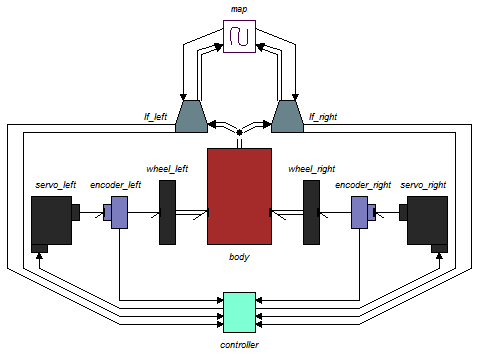
\includegraphics[width=0.6\textwidth]{lineFollowingRobot/r2g2p_ct}
\end{center}
\caption{Continuous-time model of the R2-G2P}
\label{fig:r2g2p_studyCT}
\end{figure}

The line-following sensor (seen at the top of Figure~\ref{fig:r2g2p_studyCT}) take the position and orientation from the \emph{body} block and calculate their position in the world using the \texttt{line\_follow\_x} and \texttt{line\_follow\_y} shared design parameters. This position information is passed to the map block, which takes a sample of values and passes a raw reading back to the sensors. The sensors then convert this to an 8-bit value, taking into account realistic behaviours: ambient light levels, a delayed response to changes, and A/D conversion noise.

The line-following sensor blocks also include a block to model a ``stuck'' failure (\emph{stuck\_fault}). This block has two implementations: the default (\emph{no\_fault}) does nothing to the signal and has an empty icon. The alternative is called (\emph{fail\_fixed\_value}) and has a thick, red outline and causes the sensor to always yield a fixed value (the stuck values are defined in the \emph{globals} block).

If the \emph{fail\_fixed\_value} implementation is selected in the left sensor, then it will fail after 12 seconds, always yielding 0 (black). If the \emph{fail\_fixed\_value} implementation is selected in the right sensor, it will fail when the value \texttt{lf\_right\_stuck\_value} is changed from -1 to a value between 0 and 255 by a script. The sensor will then yield whatever value is set, so this sensor can be made to get stuck on white, for example.


\section{Usage}

The line-following robot model is a good opportunity to see how
\DESTECS can support design space exploration.  A good starting point
is to run the co-model (using the \texttt{LineFollowingRobot} launch configuration), examining the speed and accuracy (distance)
with which it can complete various lines. You can then run the \texttt{LineFollowingRobot\_Outside} launch, in which the shared design parameter \texttt{line\_follow\_x} has been increased so that the sensors are ``outside'' the line on either side. Note how the simple line-following algorithm still works.

Next you can try your own combinations by altering \texttt{line\_follow\_x} and \texttt{line\_follow\_y} and observing the results. The robot generally needs to be able to distinguish when it has encountered the end of the line, and when it has encountered a sharp angle that may take the line behind its
current field of view.  Changing the forward/back position of the
sensors may make this task easier or more difficult, whilst changing
the width between the two sensors also has an impact, by altering the
resolution of the information which can be gathered about the line.

To try various designs automatically, you can define an ``ACA Launch'' configuration. Select \texttt{LineFollowingRobot} as the ``Base Configuration'', then on the ``SDPs Sweep'' tab, then try the following values: \texttt{line\_follow\_x} from 0.01 to 0.05 by 0.02, and \texttt{line\_follow\_y} from 0.01 to 0.13 by 0.06. The \DESTECS tool will then run 9 co-simulations generated from the above numbers.

Beyond this step, you could try to improve the robot's line-following. First, you could change \texttt{fast\_wheel\_speed} and \texttt{slow\_wheel\_ratio} (between 0.0 and 1.0) to alter the controller aggression. The robot could be made to drive more smoothly if a \emph{proportional} control mode was used, which applies more or less turn depending on how far from the line it is. You could change the \texttt{FollowMode} class, or create you own class and instantiate it in the constructor of \texttt{LineFollower} class.

Increasing the number of sensors would also allow for performance improvements. You can duplicate a sensor in the CT model and connect it up. You would need to alter the \emph{map} and \emph{controller} blocks to handle the new signals; instantiate more sensor objects in the DE model and make them accessible to the modes; and add a new entry to the contract / \texttt{vdm.link} file. Chapter \ref{chap:summerschoolmodels} describes five
different models of a similar line-following robot, each exhibiting
different design choices in terms of number and position of sensors,
as well as different methods for identifying the line against a
undetermined background.
